\section{Engrenagens}

Engrenagens são componentes mecânicos com a função de transmissão de potência, torque e velocidade.

A transmissão de potência através de engrenagens é um dos métodos mais fundamentais em sistemas rotodinâmicos, garantindo acoplamento cinemático rigoroso entre eixos. A geometria do dente, predominantemente modelada pelo perfil evolvente, garante uma relação de transmissão constante mesmo sob pequenas variações radiais entre os centros das engrenagens \cite{shigley2011, norton2013}.

\subsection{Geometria de Engrenagens}

A geometria básica de uma malha de engrenamento (pinhão e coroa) é definida por parâmetros primários: o número de dentes ($Z$), o módulo ($m$), o ângulo de pressão normal ($\alpha_0$) e o ângulo de hélice ($\beta_h$). A partir destes, derivam-se parâmetros fundamentais como o diâmetro primitivo ($d_p = m Z$) e o raio de base ($R_b$), dado por:
\begin{equation}
	R_b = R_p \cos(\alpha_0)
\end{equation}
onde $R_p = d_p / 2$. O contato mecânico ocorre ao longo da linha de ação, e a curva do perfil do dente é descrita pela função evolvente (involuta), matematicamente definida por:
\begin{equation}
	\text{inv}(\alpha) = \tan(\alpha) - \alpha
\end{equation}
Uma métrica fundamental do engrenamento é a razão de contato ($\epsilon$), que expressa o número médio de pares de dentes que suportam a carga em um dado instante de tempo. Ela é calculada através da intersecção dos diâmetros de adendo ($R_a$) e a linha de ação:
\begin{equation}
	\epsilon = \frac{\sqrt{R_{a1}^2 - R_{b1}^2} + \sqrt{R_{a2}^2 - R_{b2}^2} - a_w \sin(\alpha)}{\pi m \cos(\alpha_0)}
\end{equation}
onde $a_w$ é a distância real de operação entre os centros geométricos e os índices 1 e 2 denotam o pinhão e a coroa, respectivamente.

\section{Modelagem Dinâmica e Acoplamento de Rotores}
A incorporação da dinâmica de engrenamentos na análise de rotores exige que os subsistemas individuais sejam acoplados nas matrizes globais (massa, amortecimento, rigidez e giroscópica).

Em sistemas tridimensionais, onde cada nó da malha possui seis graus de liberdade (translações $x, y, z$ e rotações $\theta_x, \theta_y, \theta_z$), a formulação das matrizes de acoplamento deve decompor a força de contato normal na linha de ação considerando a cinemática 3D \cite{stringer2008}. Isso forma submatrizes interconectadas ($K_{ii}, K_{jj}, K_{ji}, K_{ij}$) que relacionam vibrações laterais e torcionais através da projeção vetorial governada pelo ângulo de pressão ($\alpha_0$), o ângulo de hélice ($\beta_h$) e o ângulo de orientação espacial do acoplamento ($\phi$).


\subsection{Rigidez de Acoplamento de Rotores Engrenados}

Para realizar o movimento conjunto entre os rotores motor e movido, é necessário acoplar as matrizes dos dois rotores nos graus de liberdade correspondentes dos nós correspondentes, representados por $q_i$ e $q_j$. Dessa maneira, a equação do movimento pode ser modificada para Eq.~\ref{Eq:mov-alt}, já contemplando a massa, rigidez e amortecimento dos dois rotores. A Fig.~\ref{fig:mesh_repr} representa esquematicamente o engrenamento, mostrando que a rigidez de acoplamento das engrenagens $K_{mesh}$ é na direção da linha de ação e não na linha que liga os centros das duas engrenagens. A matriz de acoplamento da rigidez $[K_{mesh}]$ pode ser escrita de acordo com Eq.~\ref{Eq:k_mesh} \cite{stringer2008}. A Fig.~\ref{fig:gear_repr} apresenta a representação do par engrenado em elementos finitos. As matrizes $K_{ii}$, $K_{ij}$, $K_{ji}$ e $K_{jj}$ são apresentadas na Eq.~\ref{eq:k_matrices} de acordo com \citeonline{stringer2008}.

\begin{figure}
	\centering
	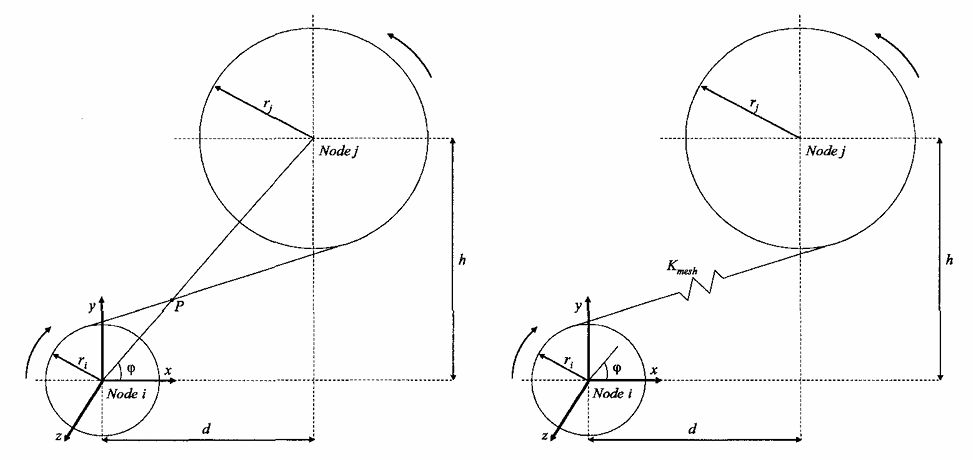
\includegraphics[width=0.8\linewidth]{figuras/gear_mesh_spring.png}
	\caption{Reapresentação do Engrenamento \cite{kaplan2012}}
	\label{fig:mesh_repr}
\end{figure}

\begin{figure}
	\centering
	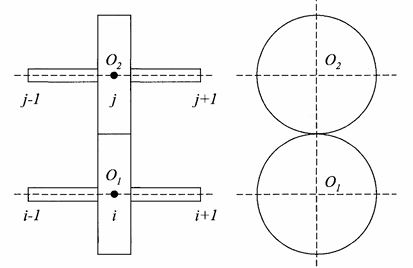
\includegraphics[width=0.6\linewidth]{figuras/gear_repr.png}
	\caption{Representação do par engrenado em elementos finitos \cite{stringer2008}}
	\label{fig:gear_repr}
\end{figure}



\begin{equation}
	[M]\{\ddot{q}(t)\}+([C]+\Omega [G])\{\dot{q}(t)\}+([K] + [K_{mesh}])\{q(t)\}=\{F(t)\}
	\label{Eq:mov-alt}
\end{equation}
\begin{equation}
	[K_{mesh}]
	\begin{Bmatrix}
		q_i \\
		q_j
	\end{Bmatrix}
	= K_{g}
	\begin{bmatrix}
		[K_{ii}] & [K_{ij}] \\
		[K_{ji}] & [K_{jj}]
	\end{bmatrix}
	\begin{Bmatrix}
		q_i \\
		q_j
	\end{Bmatrix}
	\label{Eq:k_mesh}
\end{equation}

\begin{equation}
	\label{eq:k_matrices} % Adiciona um rótulo para referenciar o conjunto de equações
	\begin{gathered}
		\resizebox{0.9\linewidth}{!}{
			$[K_{ii}] = 
			\begin{bmatrix}
				(s\phi_c\phi_x + c\phi_c\phi_x)^2 & (s\phi_c\phi_x + c\phi_c\phi_x)(s\phi_c\phi_y - c\phi_c\phi_x) & c\phi_z(s\phi_c\phi_x + c\phi_c\phi_x) & & & & \text{sym} \\
				(s\phi_c\phi_c + c\phi_c\phi_c)^2 & (s\phi_c\phi_c + c\phi_c\phi_c)(s\phi_c\phi_y - c\phi_c\phi_x) & c\phi_z(s\phi_c\phi_c + c\phi_c\phi_c) & & & \\
				c\phi_z(s\phi_c\phi_x + c\phi_c\phi_x) & c\phi_z(s\phi_c\phi_y - c\phi_c\phi_x) & c\phi_z^2 & c^2\phi_c^2r_i^2 & & \\
				-c\phi_c\phi_x r_i (s\phi_c\phi_x + c\phi_c\phi_x) & -c\phi_c\phi_x r_i (s\phi_c\phi_y - c\phi_c\phi_x) & -c\phi_c\phi_x c\phi_z r_i & s\phi_c^2 c\phi_z^2 r_i^2 & c\phi_c^2 c\phi_z^2 r_i^2 & \\
				-c\phi_c\phi_c r_i (s\phi_c\phi_x + c\phi_c\phi_x) & -c\phi_c\phi_c r_i (s\phi_c\phi_y - c\phi_c\phi_x) & -c\phi_c\phi_c c\phi_z r_i & s\phi_c^2 c\phi_z^2 r_i^2 & c\phi_c^2 c\phi_z^2 r_i^2 & c\phi_c^2 c\phi_z^2 r_i^2 \\
				-c\phi_c\phi_x r_i & -c\phi_c\phi_c r_i & -c\phi_c\phi_z r_i & -s\phi_c\phi_x c\phi_z^2 r_i & -s\phi_c\phi_c c\phi_z^2 r_i & c\phi_c^2 c\phi_z^2 r_i^2 \\
			\end{bmatrix}$
		}
		\\[1.5em] % Aumentei o espaçamento entre as matrizes para melhor leitura
		\resizebox{0.9\linewidth}{!}{
			$[K_{ij}] = 
			\begin{bmatrix}
				-(s\phi_c\phi_x + c\phi_c\phi_y)^2 & -c\phi_c\phi_z(s\phi_c\phi_x + c\phi_c\phi_y) & [K_{ij}]_{1,1} & [K_{ij}]_{3,1} & & \\
				-(s\phi_c\phi_y + c\phi_c\phi_y)^2 & -(s\phi_c\phi_y - c\phi_c\phi_x)^2 & [K_{ij}]_{1,2} & [K_{ij}]_{3,2} & -c\phi_c\phi_x r_i(s\phi_c\phi_x + c\phi_c\phi_y) & \\
				-c\phi_c\phi_z(s\phi_c\phi_y + c\phi_c\phi_y) & -c\phi_c\phi_z(s\phi_c\phi_y - c\phi_c\phi_x) & -c\phi_c^2 & -c\phi_c^2 r_j & c\phi_c^2 r_i & s\phi_c^2 c\phi_z^2 r_j \\
				-s\phi_c\phi_z^2 r_j & s\phi_c\phi_x c\phi_z r_j & -c\phi_c\phi_y r_j(s\phi_c\phi_y - c\phi_c\phi_x) & -c\phi_c^2 r_j & -c\phi_c\phi_x^3 r_i & -c\phi_c^2 c\phi_z^2 r_i \\
				c\phi_c\phi_x r_i(s\phi_c\phi_x + c\phi_c\phi_y) & c\phi_c\phi_x r_i(s\phi_c\phi_y - c\phi_c\phi_x) & c\phi_c\phi_x c\phi_z r_i & -c\phi_c^2\phi_x c\phi_z r_i & c\phi_c\phi_x c\phi_z r_j & -s\phi_c^2 c\phi_z^2 r_i r_j \\
				c\phi_c\phi_c r_i(s\phi_c\phi_x + c\phi_c\phi_y) & c\phi_c\phi_c r_i(s\phi_c\phi_y - c\phi_c\phi_x) & c\phi_c\phi_c c\phi_z r_i & -c\phi_c^2\phi_c c\phi_z r_i & c\phi_c\phi_c c\phi_z r_j & c\phi_c^2 c\phi_z^2 r_i r_j \\
				c\phi_c\phi_z r_i & -c\phi_c\phi_z r_i & -c\phi_c^2\phi_z r_i & -c\phi_c^2\phi_z r_j & -c\phi_c^2\phi_z r_i r_j & -c\phi_c^2\phi_z r_i r_j
			\end{bmatrix}$
		}
		\\[1.5em]
		\resizebox{0.9\linewidth}{!}{
			$[K_{jj}] = 
			\begin{bmatrix}
				(s\phi_c\phi_x + c\phi_c\phi_x)^2 & (s\phi_c\phi_x + c\phi_c\phi_x)(s\phi_c\phi_y - c\phi_c\phi_x) & c\phi_z(s\phi_c\phi_x + c\phi_c\phi_x) & & & & \text{sym} \\
				(s\phi_c\phi_c + c\phi_c\phi_c)^2 & (s\phi_c\phi_c + c\phi_c\phi_c)(s\phi_c\phi_y - c\phi_c\phi_x) & c\phi_z(s\phi_c\phi_c + c\phi_c\phi_c) & & & \\
				c\phi_z(s\phi_c\phi_x + c\phi_c\phi_x) & c\phi_z(s\phi_c\phi_y - c\phi_c\phi_x) & c\phi_z^2 & c^2\phi_c^2r_j^2 & & \\
				-c\phi_c\phi_x r_j (s\phi_c\phi_x + c\phi_c\phi_x) & -c\phi_c\phi_x r_j (s\phi_c\phi_y - c\phi_c\phi_x) & -c\phi_c\phi_x c\phi_z r_j & s\phi_c^2 c\phi_z^2 r_j^2 & c\phi_c^2 c\phi_z^2 r_j^2 & \\
				-c\phi_c\phi_c r_j (s\phi_c\phi_x + c\phi_c\phi_x) & -c\phi_c\phi_c r_j (s\phi_c\phi_y - c\phi_c\phi_x) & -c\phi_c\phi_c c\phi_z r_j & s\phi_c^2 c\phi_z^2 r_j^2 & c\phi_c^2 c\phi_z^2 r_j^2 & c\phi_c^2 c\phi_z^2 r_j^2 \\
				-c\phi_c\phi_x r_j & -c\phi_c\phi_c r_j & -c\phi_c\phi_z r_j & -s\phi_c\phi_x c\phi_z^2 r_j & -s\phi_c\phi_c c\phi_z^2 r_j & c\phi_c^2 c\phi_z^2 r_j^2 \\
			\end{bmatrix}$
		}
	\end{gathered}
\end{equation}

\begin{align*}
	s\varphi &= \sin\varphi, & s\varphi^2 &= (\sin\varphi)^2 \\
	c\varphi &= \cos\varphi, & c\varphi^2 &= (\cos\varphi)^2
\end{align*}

\begin{align*}
	\cos\phi_x &= \cos\beta_h \cos\alpha_n & \cos\phi_y &= \sin\alpha_n &   \cos\phi_z &= \sin\beta_h \sin\alpha_n
\end{align*}

As variáveis $q$ indicam as coordenadas generalizadas, os índices $i$ e $j$ representam os índices dos nós onde as engrenagens estão posicionadas. O parâmetro $\varphi$ representa o ângulo de orientação entre as engrenagens, $\beta_h$ é o ângulo de hélice das engrenagens e $\alpha_n$ representa o ângulo de pressão normal do par engrenado. Os ângulos $\phi_x$, $\phi_y$ e $\phi_z$ são de acordo com a Fig.~\ref{fig:force_component}, que representa a decomposição das forças no ponto de contato das engrenagens \cite{kaplan_paper_2013}.

\begin{figure}
	\centering
	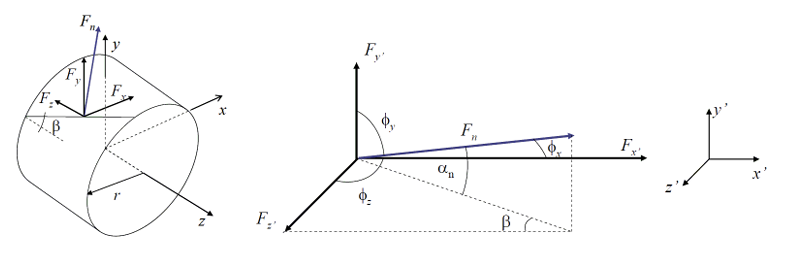
\includegraphics[width=0.9\linewidth]{figuras/force_component.png}
	\caption{Decomposição das forças no ponto de contato das engrenagens.}
	\label{fig:force_component}
\end{figure}

O parâmetro $K_g$ representa a rigidez do par engrenado ao longo da linha de ação. \citeonline{kaplan_paper_2013} apresenta uma metodologia de cálculo com base em parâmetros geométricos e do material das engrenagens, apresentada na Eq.~\ref{Eq:Kg}. Neste caso, é assumida a hipótese de que a rigidez dos dentes é mais significativa do que a rigidez do corpo da engrenagem.

\begin{equation}
	K_g = \frac{c w E_1 E_2}{9(E_1+E_2)}
	\label{Eq:Kg}
\end{equation}

Onde $c$ representa a razão de contato do par engrenado, $w$ descreve a largura dos dentes das engrenagens, $E_1$ e $E_2$ são os módulos de elasticidade das engrenagens motriz e movida, respectivamente. 

Vale lembrar que, devido à dinâmica do contato entre  os dentes, a rigidez associada ao engrenamento, na realidade, é uma grandeza variável no tempo e dependente da  razão de contato entre as engrenagens. Abaixo será apresentado  a primeira metodologia encontrada na literatura (Perfil Retangular) e o modelo completo  atualmente utilizado.


\subsection{Perfil Retangular de Rigidez de Engrenamento}

Além disso, uma simplificação muito comum quando se trata de análise dinâmica da rigidez do engrenamento é a consideração do perfil de rigidez como uma onda retangular assim como proposta por \citeonline{lin2002}.


\begin{figure}[H]
	\centering
	\caption{Perfil de rigidez do engrenamento correlacionado com razao de contato}
	\label{fig:rig_engr}
	
	\begin{minipage}{0.7\textwidth}
		\centering
		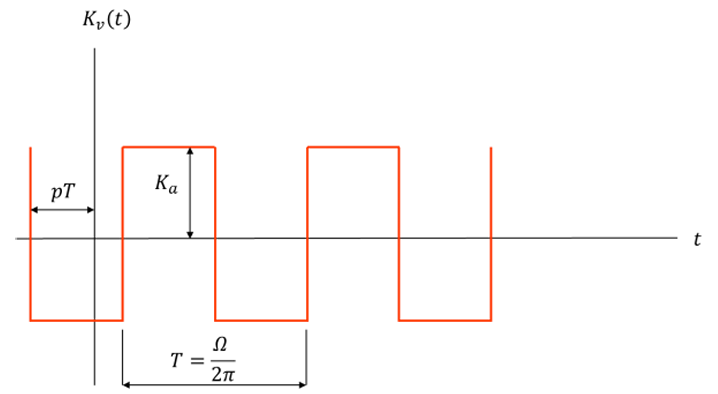
\includegraphics[width=\linewidth]{figuras/kv_kaplan}
		\par\vspace{0.3em}
		\raggedright
		{\small Fonte: \citeonline{kaplan2015}}
	\end{minipage}
\end{figure}

\begin{figure}[H]
	\centering
	\caption{Perfil de rigidez do engrenamento correlacionado com razao de contato}
	\label{fig:rig_engr}
	
	\begin{minipage}{0.7\textwidth}
		\centering
		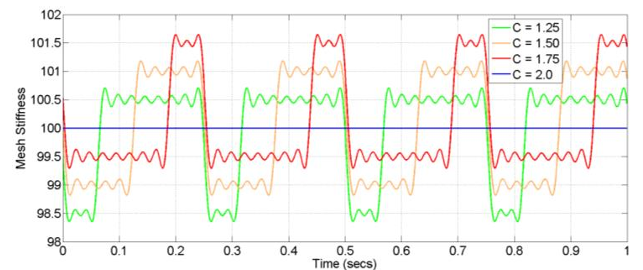
\includegraphics[width=\linewidth]{figuras/tvms_ret_kaplan}
		\par\vspace{0.3em}
		\raggedright
		{\small Fonte: \citeonline{kaplan2015}}
	\end{minipage}
\end{figure}

\begin{equation} \label{eq:stiffness_K}
	K = K_g + K_v(\Omega, t)
\end{equation}

\begin{equation} \label{eq:stiffness_Kv}
	K_v(t) = 2K_a \sum_{s=1}^{\infty} \left( a^{(s)} \sin(sN_i\Omega_i t) + b^{(s)} \cos(sN_i\Omega_i t) \right)
\end{equation}

\begin{align} \label{eq:coeficientes_ab}
	a^{(s)} &= -\frac{2}{s\pi} \sin[s\pi(c - 2p)] \sin(s\pi c) \nonumber \\
	b^{(s)} &= -\frac{2}{s\pi} \cos[s\pi(c - 2p)] \sin(s\pi c)
\end{align}


\subsection{Perfil Completo de Rigidez de Engrenamento}

O acoplamento entre duas engrenagens gera uma rigidez de malha que deve ser contabilizada na dinâmica do sistema rotativo em questão, assim como visto anteriormente. Essa rigidez, entretanto, não apresenta um valor constante no tempo e pode ser definida por um perfil de  rigidez variável assim como descrito por \citeonline{ma2014}. A Figura \ref{fig:rig_engr} apresenta o comportamento deste perfil de rigidez.

\begin{figure}[H]
	\centering
	\caption{Perfil de rigidez do engrenamento}
	\label{fig:rig_engr}
	
	\begin{minipage}{0.5\textwidth}
		\centering
		
\includegraphics[width=\linewidth]{figuras/filler_jacare_faso.png}
		\par\vspace{0.3em}
		\raggedright
		{\small Fonte: REFERENCIAAAAAAAAA}
	\end{minipage}
\end{figure}

O formato característico desse perfil tem origem da geometria do dente da engrenagem e do comportamento da malha de engrenamento. Como o perfil do dente não apresenta seção transversal uniforme a rigidez do engrenamento é alterada a cada passo de tempo devido ao contato entre os dentes acontecer em regiões de alteração da área de seção \cite{ma2014}. A Equação \ref{eq:calc_k} descreve que a rigidez associada ao engrenamento é calculada a partir da associação de rigidezes, onde $k_h$ é a Rigidez de Contato de Hertz, $k_b$ é a Rigidez à Flexão, $k_s$ ao Cisalhamento e $k_a$ à Compressão Axial. Adicionalmente, $k_f$ incorpora a rigidez do pé do dente na conexão com o corpo da engrenagem \cite{ma2014}. Tal calculo é feito a partir de métodos analíticos com base na energia potencial

\begin{equation}
	\frac{1}{k_{g}} = \frac{1}{k_h} + \sum \left( \frac{1}{k_b} + \frac{1}{k_s} + \frac{1}{k_a} + \frac{1}{k_f} \right)
	\label{eq:calc_k}
\end{equation}

--------------------------------------------------------------

\begin{figure}[H]
	\centering
	\caption{Modelo geométrico do perfil do dente da engrenagem}
	\label{fig:rig_engr}
	
	\begin{minipage}{0.5\textwidth}
		\centering
		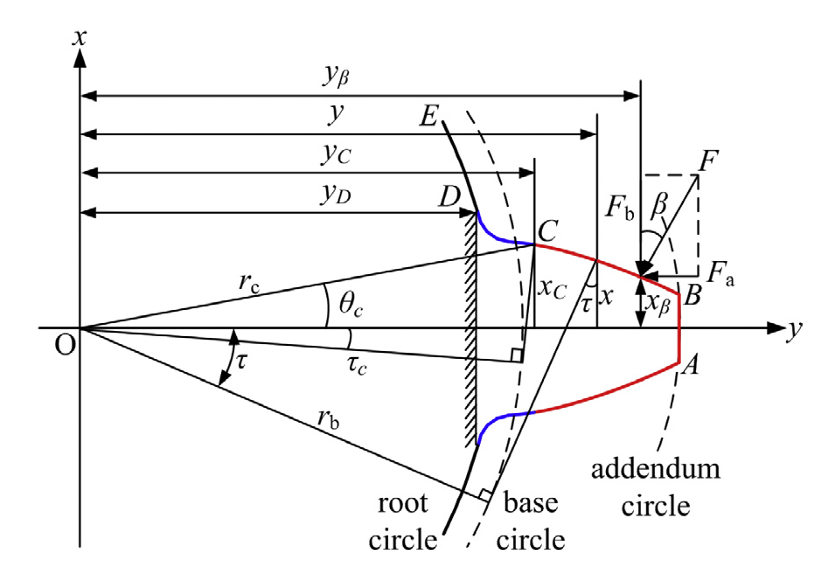
\includegraphics[width=\linewidth]{figuras/ma_gear_model.png}
		\par\vspace{0.3em}
		\raggedright
		{\small Fonte: \citeonline{ma2014}}
	\end{minipage}
\end{figure}


\begin{equation} \label{eq:componentes_energia}
	U_h = \frac{F^2}{2k_h}, \ U_b = \frac{F^2}{2k_b}, \ U_s = \frac{F^2}{2k_s}, \ U_a = \frac{F^2}{2k_a}, \ U_f = \frac{F^2}{2k_f},
\end{equation}

\begin{align} \label{eq:energia_total}
	U &= \frac{F^2}{2k} = U_h + U_{b1} + U_{s1} + U_{a1} + U_{f1} + U_{b2} + U_{s2} + U_{a2} + U_{f2} \nonumber \\
	&= \frac{F^2}{2} \left( \frac{1}{k_h} + \frac{1}{k_{b1}} + \frac{1}{k_{s1}} + \frac{1}{k_{a1}} + \frac{1}{k_{f1}} + \frac{1}{k_{b2}} + \frac{1}{k_{s2}} + \frac{1}{k_{a2}} + \frac{1}{k_{f2}} \right),
\end{align}

\begin{equation} \label{eq:rigidez_malha}
	k = \frac{1}{\frac{1}{k_h} + \frac{1}{k_{b1}} + \frac{1}{k_{s1}} + \frac{1}{k_{a1}} + \frac{1}{k_{f1}} + \frac{1}{k_{b2}} + \frac{1}{k_{s2}} + \frac{1}{k_{a2}} + \frac{1}{k_{f2}}}.
\end{equation}

\begin{equation} \label{eq:kh}
	k_h = \frac{\pi E L}{4(1 - \nu^2)},
\end{equation}

\begin{equation} \label{eq:kf}
	\frac{1}{k_f} = \frac{\cos^2 \beta}{EL} \left\{ L^* \left(\frac{u_f}{S_f}\right)^2 + M^* \left(\frac{u_f}{S_f}\right) + P^*(1 + Q^* \tan^2 \beta) \right\},
\end{equation}

\begin{equation} \label{eq:Ua}
	U_a = \frac{F^2}{2k_a} = \int_{y_D}^{y_C} \frac{F_a^2}{2EA_{y1}} dy_1 + \int_{y_C}^{y_\beta} \frac{F_a^2}{2EA_{y2}} dy_2,
\end{equation}

\begin{equation} \label{eq:Ub}
	U_b = \frac{F^2}{2k_b} = \int_{y_D}^{y_C} \frac{M_1^2}{2EI_{y1}} dy_1 + \int_{y_C}^{y_\beta} \frac{M_2^2}{2EI_{y2}} dy_2,
\end{equation}

\begin{equation} \label{eq:Us}
	U_s = \frac{F^2}{2k_s} = \int_{y_D}^{y_C} \frac{1.2F_b^2}{2GA_{y1}} dy_1 + \int_{y_C}^{y_\beta} \frac{1.2F_b^2}{2GA_{y2}} dy_2,
\end{equation}

\begin{equation} \label{eq:inv_ka}
	\frac{1}{k_a} = \int_{\frac{\pi}{2}}^{\alpha} \frac{\sin^2 \beta}{EA_{y1}} \frac{dy_1}{d\gamma} d\gamma + \int_{\tau_c}^{\beta} \frac{\sin^2 \beta}{EA_{y2}} \frac{dy_2}{d\tau} d\tau,
\end{equation}

\begin{equation} \label{eq:inv_kb}
	\frac{1}{k_b} = \int_{\frac{\pi}{2}}^{\alpha} \frac{[\cos \beta(y_\beta - y_1) - x_\beta \sin \beta]^2}{EI_{y1}} \frac{dy_1}{d\gamma} d\gamma + \int_{\tau_c}^{\beta} \frac{(\cos \beta(y_\beta - y_2) - x_\beta \sin \beta)^2}{EI_{y2}} \frac{dy_2}{d\tau} d\tau,
\end{equation}

\begin{equation} \label{eq:inv_ks}
	\frac{1}{k_s} = \int_{\frac{\pi}{2}}^{\alpha} \frac{1.2 \cos^2 \beta}{GA_{y1}} \frac{dy_1}{d\gamma} d\gamma + \int_{\tau_c}^{\beta} \frac{1.2 \cos^2 \beta}{GA_{y2}} \frac{dy_2}{d\tau} d\tau,
\end{equation}

-------------------------------------------------------------

A periodicidade característica e a amplitude deste perfil tem correlação com a razão de contato do par engrenado que define a média de pares de dentes em contato. Quando há somente um par de dentes em contato a rigidez assume a região de menor valor. Ao passo que, quando há dois pares de dentes em contato as rigidezes se somam e, portanto, o perfil de rigidez apresenta a região de maior valor  assim como apresentado por \citeonline{lais2022} e \citeonline{chico2025}.

\begin{figure}[H]
	\centering
	\caption{Perfil de rigidez do engrenamento correlacionado com razao de contato}
	\label{fig:rig_engr}
	
	\begin{minipage}{0.5\textwidth}
		\centering
		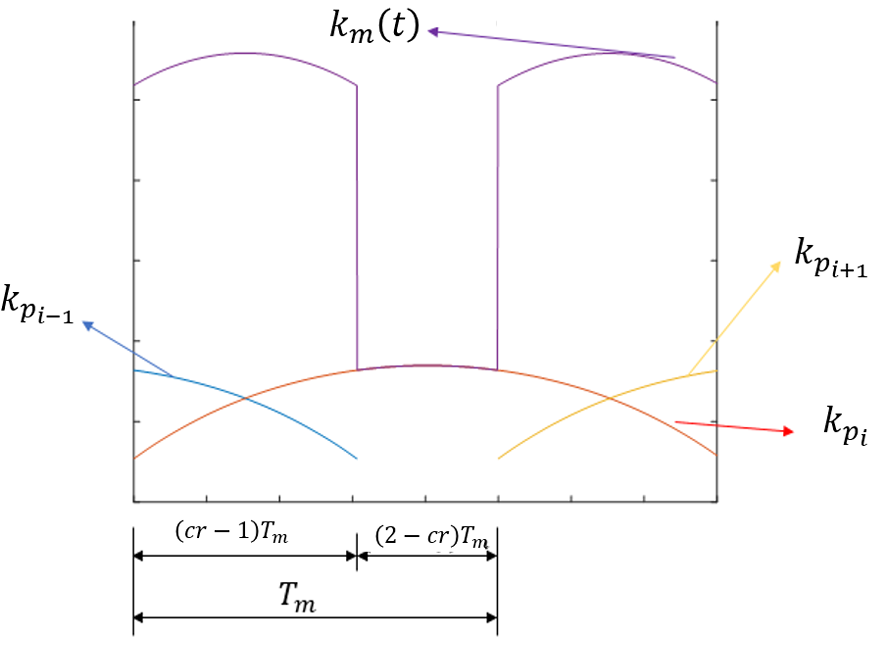
\includegraphics[width=\linewidth]{figuras/cr_km.png}
		\par\vspace{0.3em}
		\raggedright
		{\small Fonte: \citeonline{lais2022}}
	\end{minipage}
\end{figure}

